%-----------------------------------------------------------------------------
%
%          PHYSICS  M.S.     THESIS
%          JUSTIN A. VASEL
%
%          This began as the template offered by the University of Minnesota, 
%          but I've made a few changes here and there...  
%
%          -->  halo2.tex
%
%-----------------------------------------------------------------------------


\chapter{The Road to Full Operation}
	\label{halo2_chapter}

	\begin{quoting}
		\noindent \large ``For tomorrow belongs to the people who prepare for it today." \normalsize

		--- African Proverb
	\end{quoting}

	\chapterIntro{I}{arrived at SNOLAB to begin work on HALO in July of 2012.} Construction of the detector hardware had finished not long before that and the detector had been running and collecting data since May of 2012. However, HALO was far from being ready to do its job. Many vital components were missing: SNEWS alert triggers were not developed, hardware redundancy was not in place, there was no way to remotely monitor the hardware, and the detector had not yet been calibrated. 

	My work at HALO was not singularly data analysis nor theoretical research nor computer simulation. My contribution to the experiment was more vague and arguably more involved: to help the collaboration move through this laundry list of tasks in a timely manner so that HALO will be ready to serve its purpose before the next galactic supernova occurs. In this chapter, I will discuss my involvement in preparing the Helium and Lead Observatory for full operation.

	\section{Identifying Faulty{}\he Counters}
		As mentioned in \CHP \ref{halo_chapter}, the{}\he proportional counters were donated to HALO by the decommissioned SNO experiment. Only 128 counters are required for HALO, which left us with a couple dozen extra to be kept on reserve in case a counter in the detector for whatever reason needs to be replaced. The neutron spectrum for each counter currently in the detector had been carefully examined to ensure the active counters were behaving as expected, but the extra counters had not yet been so thoroughly vetted. It was known that some of the counters were filled with $^4$He gas, which cannot be used in the detection of neutrons. The SNO experiment used these as a control group and they got mixed in with the{}\he counters when they were delivered to HALO. 

		To identify the $^4$He counters in the group and to ensure that the{}\he counters were behaving normally, we tested each of them by collecting and examining their neutron spectrum. To avoid disrupting any of the 128 active counters in the detector during testing, we ran wiring from the storage rack to the rest of the hardware. This allowed us to test four counters at a time while the rest of the detector ran normally.

		Most counters were allowed to accumulate data for several days before inspection. A healthy{}\he counter displayed a statistically significant neutron peak located near an ADC value of 1,000\footnote{At this point, the arbitrary ADC value scale for energy had not been mapped to keV. Such a mapping depends on the peculiarities of the{}\he counter, the gains within it, and thresholds applied to it. An algorithm to perform this conversion for each counter is currently in development.} and a tall and sharp gamma peak at very low energies (\FIG \ref{fig:halo_neutron_spectra}, left). An unhealthy{}\he counter may have a broadened neutron peak or other strange artifacts in the spectrum (\FIG \ref{fig:halo_neutron_spectra}, center). A $^4$He counter would simply not have the neutron peak (\FIG \ref{fig:halo_neutron_spectra}, right).
		\begin{figure}[H]
			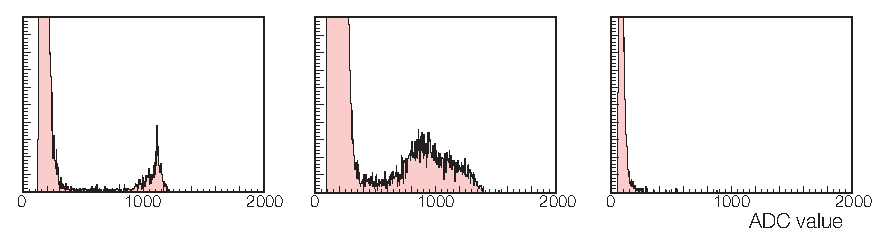
\includegraphics[width=\textwidth]{halo_neutron_spectra}
			\caption[Neutron Counter Response]{\bf Neutron counter response. \rm A healthy{}\he counter \emph{(left)} exhibits a sharp neutron peak and a gamma peak. An unhealthy{}\he counter \emph{(center)} also has a gamma peak, but may show a broadened neutron peak or other obscure features. A $^4$He counter \emph{(right)} features a gamma peak, but no neutron peak.}
		\label{fig:halo_neutron_spectra}
		\end{figure}

		The $^4$He counters are not completely useless to the experiment, however. As discussed in \SEC \ref{sec:noise}, gamma rays produced by the nuclear decay of uranium and thorium daughters in the lead paint can Compton scatter with electrons in the tubes and ionize the surrounding gas. There is no neutron capture processed involved in that case, so both \he and $^4$He counters can detect gamma rays. These counters may be used to study the gamma backgrounds in an effort to separate them from the neutron peaks in the \he counters. 

		After characterization, we identified both healthy and unhealthy{}\he counters and the $^4$He counters. A \he counter with a gas leak will experience either a decrease or increase in gain, depending on how much gas has leaked, and manifest itself as a distorted neutron spectrum. We suspected that any unhealthy spectra we found would be due to such a leak, but after finding several of these, we began to wonder if there was another explanation. It was a symptom worthy of further investigation, in case it represented a larger problem that could affect healthy{}\he detectors down the road.

		It was suggested that perhaps the electrical connection between the anode wire and the endcap that connects it to the high voltage was not sound. The endcaps connect to the anode wire through a small metal spring. At the end of the spring is a ball that fits into a socket at the end of the anode wire. We imagined two scenarios that might degrade the electrical connection: the ball on the spring did not fit into the socket and is instead resting on the side of the anode wire; or the spring has lost compression over time and is no longer making firm electrical contact.

		To test these ideas, we began removing endcaps from the detectors in question and examining the connections. There was no evidence of any of the springs being bent, but the possibility of them having lost sufficient compression to provide a good electrical contact was still plausible. We placed a small dab of conductive grease to the end of the spring ball to provide a strong electrical pathway even if ball and socket were only barely touching. 

		This did not make a difference; the spectra still appeared deformed. Since we tried improving the connection with conductive grease, others have attempted to measure how the spring compression changes over time. They found that the springs do tend to loose compression very quickly. A spring compressed by \SI{4}{\milli\metre} lost much of its compression within the first few minutes and approached a value of \SI{2}{\milli\metre} after a few hours. The manufacturer claims that \SI{2}{\milli\metre} is the amount of compression needed to make a strong electrical contact, so these results initially were not too concerning. However, over a longer time scale of about a week, the springs lost an addition \SI{0.5}{\milli\metre} of compression\cite{spring_test}. It is not clear whether this is the cause of the deformed neutron spectra, but it will continue to be investigated.

	\section{DAQ Software Development}
	\label{sec:orca_development}
		The HALO detector and its related hardware is monitored and controlled by a software package called ORCA (Object-oriented Real-time Control and Acquisition), developed by Mark Howe at the University of North Carolina at Chapel Hill.\footnote{http://orca.physics.unc.edu/$\sim$markhowe/} ORCA is written in Objective-C using the Cocoa framework and Apple Developer Tools. It is a powerful application, providing native support for a wide range of devices, data readout and analysis tools, and the ability to write custom processes within the software. Being well-versed on the Apple OS X operating system, it made sense for me to act as the liaison between HALO and ORCA development. 

		ORCA is open-source. It is tracked using Subversion and compiled using Apple's Xcode4 software. We wanted to have the ability to add functionality to ORCA that we needed at HALO. Before I could do that, though, I had to learn Objective-C. I hadn't done much with object-oriented languages in the past, so I found Objective-C to be quite abstract and the learning curve steep. 

		ORCA follows the Model-View-Controller paradigm. Each component of the application has associated with it at least five files. 

		\begin{verbatim}
		ExampleModel.h
		ExampleModel.m
		Example.nib
		ExampleController.h
		ExampleController.m
		\end{verbatim}

		The \verb$.h$ files are header files that describes the class interface: definition of instance variables and public methods. Implementation is contained within the \verb$.m$ files, which contains the code for the methods described in the header as well as private methods. The \verb$Model$ files contain code that store information or manipulate states. They have no connection to the user interface. \verb$Controller$ files on the other hand, are the glue that binds the models to the user interface. They ensure that changes made in the model are updated on the screen and conversely that user input gets passed to the model. Finally, the \verb$.nib$ files represent the view, the user interface. They are not coded, but instead graphically designed through Xcode's Interface Builder. 

		The \he detectors in HALO are associated with a variety of electronics and hardware. Each detector is connected to a VME crate, card and channel; a high-voltage crate and channel; a preamp; and a pulser card and channel. Furthermore, each counter has an identification number printed on it and is located at some position within the detector. Since it's likely that detectors may get shuffled around to different positions in the detector, it is important to have a record of all these pairings for future reference. This was originally achieved by including a list of all 128 detector ID numbers and their positions in the detector in a text-input box in ORCA. 

		That method could work temporarily, but in the long term a more robust archival method is necessary. With so many components that could fail, it is crucial to know what is connected to what at all times. I set out to implement a hardware map for the HALO object in ORCA that would store all of the aforementioned details for each detector in an easy to read table, and that could be exported to or imported from a Comma Separated Values (CSV) file for easy saving. 

		First, I designed the table in Xcode4. This involved partitioning a table into the right amount of columns for everything I wanted to track and assigning to each column a unique identifier that links it to a particular value from each row of the CSV file.

		\begin{figure}[H]
			\includegraphics[width=\textwidth]{orca_dev_1}
			\caption[ORCA Development: Building the Hardware Map]{\bf Building the hardware map. \rm This screenshot of Xcode shows the graphical Interface Builder that is used to design user interfaces. Halo.nib is the file being edited here. In the center of the interface is the table that will be populated with the details of the hardware map. When a CSV file containing the map is read, each column is assigned a unique identifier, which must also be assigned to a column in the table (on the right).}
			\label{fig:orca_dev_1}
		\end{figure}
		\newpage
		Building the table was done graphically, through Xcode's Interface Builder. There is no programming required to build these visual elements. But, the elements need to be linked to objects from code in order to be used. For example, to put the contents of a CSV hardware map file into the table, the user pushes the ``Read'' button and browses for the file. There is an action in the code associated with this button, which reads in the file and parses the CSV syntax. The results of that action are stored in an object that is associated with the table I created. To ensure that the correct values make it into the correct columns, the values from the file are added to a dictionary of key-value pairs. Each key is a unique identifier that is specified in the appropriate column on the table (\FIG \ref{fig:orca_dev_1}).

		\lstset{language=object-c,
		gobble=23}
		\begin{lstlisting}[escapechar=$, caption={\it HaloModel.m. \rm \\ \linespread{1} \small Code required to assign values from CSV file to keys that can be displayed in the hardware map table. Only one entry of the list is shown, but the structure is the same for all of them.} ]
			- (NSMutableArray*) setupMapEntries:(int) index
			{
			  NSMutableArray* mapEntries = [NSMutableArray array];

	          		  . . .

			  [mapEntries addObject:[NSDictionary 
			    dictionaryWithObjectsAndKeys: @"kHvCrate", 
			    @"key", [NSNumber numberWithInt:0], @"sortType", nil]];

	        		  . . .

			  return mapEntries;
			}
		\end{lstlisting}

		With the code finished, I moved on to producing the necessary CSV file for the current detector configuration. It was an exercise in tedium, following cables from the detectors to the preamps and then down to other hardware. Finally I was able to produce a document like the one below:

		\begin{verbatim}
			0,7106,0,3.00-233,8,4,0,3,H316,0,0
			1,7139,3,3.00-221,8,5,0,2,H349,0,12
			2,7106,6,3.00-160,8,4,0,3,H316,0,0
			3,7139,9,3.00-230,8,5,0,2,H349,0,12
			4,7206,0,3.00-199,8,6,0,2,H342,0,6
		\end{verbatim}

		Finally, I imported the file into ORCA to produce the table seen in \FIG \ref{fig:orca_dev_2}.

		\begin{figure}[H]
			\includegraphics[width=\textwidth]{orca_dev_2}
			\caption[ORCA Development: Completed HALO Hardware Map]{\bf Completed HALO hardware map. \rm The imported CSV file populates the table. Now the information about what is connected to what is easily accessible, easily editable, and savable as another CSV file for archiving. There is no need to edit the CSV file directly. If the detector configuration is changed, these values can simply be changed on the fly in the table.}
			\label{fig:orca_dev_2}
		\end{figure}

		HALO also has a test stand of four \he detectors outside of the main apparatus. This was developed while testing the \he tubes for defects. Later it was realized that this feature should be extended to map the test stand as well. I created a separate tab in the user interface for the test stand. I purposefully kept them in separate tables, so that it was clear which detectors were active in the experiment and which were being used diagnostically. 

		\begin{figure}[H]
			\includegraphics[width=\textwidth]{orca_dev_3}
			\caption[ORCA Development: DetectorView Improvements]{\bf DetectorView improvements \rm The DetectorView looks like the physical HALO detector. The colors represent the total counts on each \he tube during the run. This can be used as a quick inspection of relative detector response. You can see the tubes in the lower left of HALO have relatively high rates (there was a neutron source in that area). Each \he can now be selected to reveal its hardware map information (on the right).}
			\label{fig:orca_dev_3}
		\end{figure}

		There is another portion of the HALO object in ORCA that displays a cartoon graphic of the detector. It is a simple graphic, consisting of circles that represent each \he counter arranged on the screen in the same way they're arranged physically. Each circle is filled with a color that corresponds to the number of counts it has had during the current run. This view---which we call the DetectorView (\FIG \ref{fig:orca_dev_3})---is a great diagnostic tool, allowing us to immediately notice if any of the 128 detectors are acting differently from the rest. Clicking on an individual circle reveals some information about that particular detector. Originally, it only listed the shaper card and channel. I extended this to display all of the information available in the hardware map. Now, we have the ability to choose any \he detector at random and instantly know everything that it is connected to. This will make troubleshooting detector-related problems much easier.


	\section{Network Design}
		HALO is intended to operate for decades. Once it is in its final state and operating normally, there will not often be people stationed underground near the hardware. For this reason in particular, and because it's just good form generally, it is important that everything is organized in a common sense way and well-documented. As we began to add more computers to the set up, it became clear that a formal network organizational structure was necessary. 

		We have nearly two of every device on the network. This is for redundancy. It is critically important that single point of failure cannot bring HALO offline when that supernova finally occurs. I wanted to develop a networking scheme that made sense and was easy to remember. I put each device and its backup into a group, for a total of twelve groups. The exception to this rule were the two DAQ computers, which each exist in their own group, but have two network interfaces. I numbered the groups from 0--11 and assigned them private IP addresses following the scheme:
		\begin{verbatim}
		    xxx.xxx.[group number].[device number]
		\end{verbatim}
		Where \verb$xxx.xxx$ is the private network address, redacted for security purposes. For example, there are two VME crates, which belong to group number 7 on my list. Their private IP addresses, respectively, are
		\begin{verbatim}
		    xxx.xxx.7.1
		    xxx.xxx.7.2
		\end{verbatim}

		We also have machines that connected to the outside world for remote monitoring purposes. These were assigned public IP addresses by SNOLAB and don't follow any kind of formula like the private addresses, but they are at least sequential in the same direction as the private addressing scheme, making them as sensible as possible. Hostnames were also chosen for the private network. They follow a scheme very similar to that as the private IPs:
		\begin{verbatim}
		    halo-[group name][device number]
		\end{verbatim}
		So again, in the case of the two VME crates, their hostnames are:
		\begin{verbatim}
		    halo-vme1
		    halo-vme2
		\end{verbatim}

		I chose this network scheme to be simple and easy to remember. It is also extensible. In the event that a new piece of hardware is installed in the future, it can easily be assigned an IP and a hostname that conforms to this standard. Security is a concern for these devices since they have a link to the Internet that will be used for remote monitoring. Besides that one point of entry, the network is isolated on its own subnet with port forwarding carefully configured.

	\section{Remote Monitoring}
		HALO is designed to be low-maintenance. It can run continuously for long periods of time automatically. This allows for experimenters to spend most of their time on surface working on other things, rather than spending valuable time under ground running the detector. Despite the automated capacity of HALO, it is still essential to monitor the behavior of the detector in order to identify any problems that arise that would prevent HALO from triggering on a supernova signal when it comes. Such monitoring can be performed remotely, however, eliminating the need to spend time underground when the detector is functioning normally.

		There is a shift system in place, in which HALO collaborators take turns checking up on the detector. Each experimenter in the shift rotation is responsible for monitoring the detector for a block of three days at a time. During that time, they document the status of HALO by submitting an online shift report twice a day. A shift involves confirming that voltages are as expected, that the detector is in the process of collecting data, and looking for peculiarities in the accumulated data.

		The method to perform these checks currently involves connecting to the DAQ machine through a remote desktop interface. From there, the shifter has direct control over the Orca application, and thus the HALO detector itself. Aside from its usefulness for shift reports, remote desktop access has been a valuable tool while HALO was being constructed and developed, allowing us to update software and adjust detector parameters after-hours. 

		But, as HALO nears its final configuration the remote desktop method of monitoring becomes less ideal and more of a liability. It is not hard to foresee an instance in the future wherein a shifter connected via remote desktop produces an accidental click that halts the collection of data or disrupts the high voltage or shuts down the DAQ computer. There are countless things that could go wrong when people routinely directly access the DAQ remotely. For this reason, the development of a non-disruptive remote monitoring system is necessary.

		I decided to take up the development of such a system, but there were many things to consider before jumping in. HALO is very much a long-term experiment. I began by considering the following guidelines:

		\begin{enumerate}
		\item \bf Longevity. \rm HALO is a long-term experiment. It makes sense to develop a remote monitoring system that will last a long time too. The architecture used must be one that is likely to be supported by modern operating systems for years to come.
		\item \bf Simplicity. \rm Over its lifetime, the remote monitoring system will likely be used and maintained by many people. The system needs to be as simple as possible to ensure that future experimenters will be able to understand how it works and make modifications with ease.
		\item \bf Extensibility. \rm There will likely be new hardware added to the experimental configuration in the future. The remote monitoring system should be designed in a way that allows for the inclusion of new devices or functionality with ease. 
		\end{enumerate}

		Bearing those guidelines in mind, I developed a system in which Perl scripts on local machines run at specified intervals to poll the hardware and push the response into a database. Information from the database is then served to a web interface through PHP and Javascript. The shifter can then view the relevant information without having any control over the experiment. I will now describe the system in detail.

		\subsection{Data Scraping}
		Many devices involved with running HALO are connected to the private ethernet network and are accessible in some way, whether by SNMP (Simple Network Management Protocol) or telnet or some other protocol. The trick then is to extract desired information from each device automatically. This is something a script can do quite easily. For example, the VME crates are the interface between the shaper cards and ORCA, and are accessible through SNMP. A simple command is all that's necessary to extract any piece of information provided by the crate. Here's an example of some of the information it can provide us:
		\begin{verbatim}
		  outputSwitch.U0 = INTEGER: ON(1)
		  outputSwitch.U1 = INTEGER: ON(1)
		  outputSwitch.U5 = INTEGER: ON(1)
		  outputVoltage.U0 = Opaque: Float: 5.000000 V
		  outputVoltage.U1 = Opaque: Float: 12.000000 V
		  outputVoltage.U5 = Opaque: Float: 12.000000 V
		  outputAdjustVoltage.U0 = INTEGER: 0
		  outputAdjustVoltage.U1 = INTEGER: 0
		  outputAdjustVoltage.U5 = INTEGER: 0
		  outputCurrent.U0 = Opaque: Float: 115.000000 A
		  outputCurrent.U1 = Opaque: Float: 23.000000 A
		  outputCurrent.U5 = Opaque: Float: 23.000000 A
		\end{verbatim}
		I wrote a simple Perl script that uses the \verb$snmpget$ command to extract the information we're interested in monitoring. The script then arranges that information in a JSON-formatted string and pushes it to a database, but those details will be examined in the next section.

		ORCA has built within it a method for extracting relevant information as well. A socket connection can be opened that allows a script to call any function from within ORCA. This allows us to extract details like the current voltage on each HV channel, the thresholds and gains set on each shaper channel, and any other ADC value that we choose. I have not yet written the scripts that will scrape data in this way, but it is a near-future plan. Additionally, ORCA can send run-related information to a database automatically. Much of the information need for shift reports can be gathered this way. Examples include run number, elapsed run time, counts on each detector, alarms, and the status log to name a few.

		The scripts that gather the data from all these sources can be called in a couple of ways. Currently, they are run automatically every two minutes. But, they can also be called directly from the web interface if the user wants to see the updated information immediately. I chose the interval time of two minutes arbitrarily during development, so it will likely change if the temporal resolution is too low to produce a confident shift report.

		\subsection{Database Management}
		The information gathered by the data scrapers is pushed into a database. More specifically, a CouchDB\footnote{CouchDB was invented by Apache: http://couchdb.apache.org/.}. A CouchDB is a schema-less database that uses a RESTful HTTP API\footnote{RESTful APIs are controlled through HTTP methods like GET, PUT, POST, and DELETE.} for the storage and retrieval of information. The most fundamental unit in a CouchDB is called a document. A document is in some ways analogous to a table in an SQL database, only there are no predefined fields or field types. Instead, a document is simply a string formatted as JSON.

		JSON (JavaScript Object Notation) is very similar to XML in that it consists of key-value pairs, but it is designed to be human readable. An example is shown in Listing \nolinebreak \ref{lst:json}. JSON-formatted data are very versatile and easily implemented into web code with pre-existing libraries. Each document in the CouchDB has associated with it an id (\verb$_id$) and a revision number (\verb$_rev$). When updating an entry in CouchDB, the previous entry is not deleted. Instead, the updated document is stored with the same \verb$_id$ the original had, but an incremented \verb$_rev$, allowing the user of the database to keep a history of the database as time goes on. In CouchDB, nothing is ever lost. 

		\begin{lstlisting}[language=json,firstnumber=1,label=lst:json,caption=\it A JSON Example.\rm \\ Here is a short list of neutrino observatories with some descriptive attributes. This format is both human and machine readable!]
			{
			  {
			    "Name":"HALO",
			    "Location":"Canada",
			    "Type":"High-Z (Pb)"
			  },
			  {
			    "Name":"Super-Kamiokande",
			    "Location":"Japan",
			    "Type":"Water Chernekov"
			  }
			}
		\end{lstlisting}

		CouchDB's revision feature and its sans schema philosophy make it ideal for use in the HALO remote monitoring system. The revision-tracking will allow us to recall the state of the detector in the past if needed, and the lack of a rigid schema make storing new types of information painless. This flexibility will contribute to the goal of making the system extensible.

		The last thing I'll mention about CouchDB for now is that it is not accessible through a command line or a custom protocol. Rather, it is accessible through HTTP. The CouchDB server creates a web server on the default port of 5984. To retrieve a document titled ``doc" from the database called ``db'', you can simply point your web browser to http://localhost:5984/db/doc and the result will be the contents of the document as a JSON string. This simple method of access makes it easy to retrieve documents from CouchDB with any programming language that supports basic HTTP requests. 

		The data scrapers that gather information from the experimental hardware format the information as JSON before pushing it to the local CouchDB as a document. Conveniently, ORCA already includes native support for CouchDB. After writing an example data scraping script for the VME crates and setting up the databases, I had most of the basic infrastructure for the remote monitoring system in place. What remained was the development of a user interface.

		\subsection{A Simple, Yet Powerful User Interface}
		I have been able to stay true to the guidelines I set for myself during the development of the data scrapers and the database. They're simple, they're sustainable, and they're extensible. The user interface was bound to be the more difficult task in these regards. It is very easy for web code to get messy and disorganized because there is a lot of it. To avoid this, I built the code very slowly, making sure that each part of the code was separate from the others. The code to pull documents from CouchDB was separate from the code that parses the resulting JSON response, which in turn was separate from the code that prints the information to the screen. In this way, the code is modular. This will make it easy to add new code in the future. It also makes understanding how the code works much easier.

		The user interface is written in a combination of three languages commonly used in web programming. The core of the interface is written in PHP, a recursive acronym that stands for \it PHP: Hypertext Preprocessor\rm. PHP is a server-side scripting language; it gets executed on the server and the user is served the output. In this case, the PHP scripts are mainly used to request documents from the database. The JSON-formatted response is passed into the next layer of programming, Javascript, where it is parsed.

		Javascript, as opposed to PHP, is a client-side language. It is responsible for parsing the JSON received from CouchDB and performing functions on it (like formatting or calculations) before it is displayed to the user. I am using a popular Javascript library called jQuery\footnote{http://jquery.com/}, which provides a means of updating elements that have already been drawn on the web page. jQuery will allow the information on the page to be updated as the database is updated, providing the user with a nearly-live view of the detector parameters. 

		\begin{figure}[H]
			\includegraphics[width=\textwidth]{monitoring_ui}
			\caption[Prototype Remote Monitoring User Interface]{\bf Prototype remote monitoring user interface. \rm This early version of the remote monitoring tool displays a subset of the desired HALO information in a clean and easy to understand interface. The HALO DetectorView from ORCA is replicated in the lower left, although the colors which normally correspond to counts are temporarily randomized for testing purposes.}
			\label{fig:mon_ui}
		\end{figure}

		The final programming tier in the user interface is simple HTML. This language defines the structure of the web page. It dictates where the content will be placed and how it will be styled. HTML is also client-side, however it is not considered a programming language. It cannot perform calculations or understand conditional statements; It is simply a markup language. The HTML elements are known as DOM nodes and are manipulated by jQuery to present dynamic content.

		Continuing to embrace the idea of simplicity and modularity, I made use of a powerful HTML framework called Twitter Bootstrap\footnote{http://twitter.github.io/bootstrap}. This provided a basic grid layout as a skeleton and a handful of style rules to make the web page visually appealing. Using the grid layout, I was able to design a page that is visually modular. Similar components are grouped together instead of being scattered throughout the page, much like the code (\FIG \ref{fig:mon_ui}). 

		The basic infrastructure that powers the HALO Remote Monitoring Tool is currently in place. It includes automated data scrapers, a centralized database and a user interface powered by server-side, client-side, and markup languages. At the time of writing, the collaboration is in the process of deciding exactly which quantities we want to monitor with the tool. The modularity I built into the code will make that process trivial; any new code will essentially be ``plug and play". 


	\section{Current Status and Future Work}
		I will continue to develop and document the HALO Remote Monitoring Tool for the time being. I expect it to be ready for regular use during shift reports within the next month, representing a milestone in the process of bringing HALO closer to its final, steady state configuration. 

		The HALO experiment is getting close to full operations, but there are still several outstanding items on the checklist. 
		\begin{itemize}
			\item \bf Placement of front water shielding. \rm Until very recently, the \he detector pairs in HALO had not been gain matched. Since there are two detectors per channel, it is desirable for them to have as similar gains as possible so that their neutron peaks occur at the same ADC value. Now that the gain matching process is finished and the \he detectors are likely in their final configuration, the water shielding that will cover the front face of the detector can be installed. 
			\item \bf Improvement of Monte Carlo simulation. \rm HALO uses the Geant4\footnote{http://geant4.cern.ch/} software package to simulate particle behavior within the detector. A basic version of MC has been around for some time, improvements have been made to it periodically over the last year. However, there are still further improvements to be made and perhaps some bugs to work out before it will be ready for use in calibration.
			\item \bf Detector calibration. \rm The detector will be calibrated with a $^{252}$Cf neutron source. I briefly worked to characterize $^{252}$Cf neutron emission for use in the MC by referencing previously-measured $^{252}$Cf neutron spectra and multiplicities, however it appears that the Geant4 software may already have that functionality built in. The source is currently awaiting encapsulation, but will soon be underground. Calibration data-taking should begin within the next few months.
			\item \bf Isolation of the neutron peak. \rm The neutron spectrum contains a large amount of low-energy events that are caused by gamma rays Compton scattering on electrons within the detectors. This peak appears to merge with the shoulder of the neutron peak. The peaks are clearly separate from each other, but it's not clear where one ends and the other begins. This ambiguity can lead to problems with low-energy neutron detection. The best solution is to fit functions to each peak and then strategically cut as many gammas as possible without cutting any neutrons. The gamma peak is easy to fit; it is an exponential. The neutron peak---with its skewed shoulder---is more complicated, but achievable. An algorithm has already been developed to do this, but it needs improvement before it can be relied on. If the interface between gammas and neutrons can be identified for each \he detector, then the thresholds on the shaper cards can be adjusted to eliminate as many gammas as possible at no expense to the neutrons.
			\item \bf Supernova Triggers and Joining SNEWS. \rm Once the detector is fully shielded and calibrated, the supernova triggers must be developed and implemented so that HALO can become an active participant in SNEWS. To abide by the false-alarm limits set by SNEWS, HALO's triggers will listen for a burst of 6 neutron detection events in a 2 second time window. With this trigger threshold, HALO will be capable of generating a SNEWS trigger for any supernova within \SI{17.5}{\kilo\parsec} of Earth\cite{Shantz2010}: a region that encompasses most of the stars in the Milky Way.
		\end{itemize}


%-----------------------------------------------------------------------------
%-----------------------------------------------------------------------------